\section{Introduction}

This project studies a formal extension of the Cube Rule of Food, a morphology-based framework originating in Phosphatide's ``Grand Unified Theory of Food Identification''~\cite{phosphatide_gutfi} and later popularized and expanded by André Arko at \url{https://cuberule.com/}~\cite{arko_cube_rule_food}, using a rank-3 tensor $T$ over three categorical axes.
The immediate objective is to define a compact ontology in which each food is assigned a coordinate triple $(i,j,k)$ in the discrete latent space $\{1,\ldots,I\} \times \{1,\ldots,J\} \times \{1,\ldots,K\}$, so that canonical Cube Rule examples are representable and ambiguous cases are explicit.
Our framing treats occupancy, sparsity, and ambiguity as geometric properties of $T$ rather than anecdotal judgments.
Under this formulation, cuisine is represented as a discrete structure over the index space rather than as an informal list of examples.

\subsection{The Cube Rule of Food}

The Cube Rule of Food is a morphology-based classification scheme that assigns a dish according to where structural starch appears on the six faces of an idealized cube. The core idea originates with Phosphatide's ``Grand Unified Theory of Food Identification''~\cite{phosphatide_gutfi}, while the Cube Rule formulation used here follows the later presentation and elaboration by André Arko~\cite{arko_cube_rule_food}.
In the original Rule, these labels are morphology-only categories rather than cuisine names: \emph{salad} has no structural starch faces, \emph{toast} has a bottom starch face, \emph{sandwich} has top and bottom starch faces, \emph{taco} has left, right, and bottom starch faces, \emph{sushi} has top, left, right, and bottom starch faces, \emph{quiche} has side walls and a bottom with an open top, \emph{calzone} is fully enclosed, \emph{cake} consists of stacked starch layers, and \emph{nachos} denotes an outer container plus interior starch pieces.
Some of the Rule's most memorable examples are notably surprising: nigiri counts as \emph{toast}, an Uncrustable counts as \emph{calzone}, and a salad with croutons counts as \emph{nachos}; for the lettuce-crouton boundary case discussed later, see Figure~\ref{fig:horseshoe-salad}.
These nine morphologies define the cube-type axis used throughout this paper and supply the structural vocabulary that the tensor formalism extends with protein and starch-type axes.
Figure~\ref{fig:cube-rule-types} adapts the Cube Rule morphology diagram in schematic form from Arko's presentation~\cite{arko_cube_rule_food}, itself an adaptation and popularization of Phosphatide's original post~\cite{phosphatide_gutfi}.
\begin{figure*}[!tb]
\centering
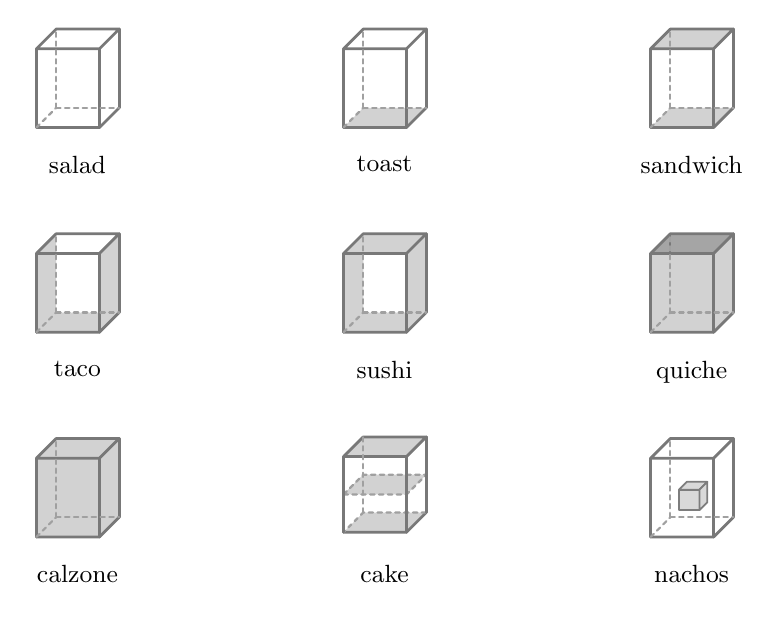
\begin{tikzpicture}[x=1cm,y=1cm,line cap=round,line join=round,font=\small]
\definecolor{starchfill}{RGB}{210,210,210}
\definecolor{starchinner}{RGB}{165,165,165}
\definecolor{starchdark}{RGB}{125,125,125}
\definecolor{wiregray}{RGB}{120,120,120}

\newcommand{\cubehidden}{
  \draw[wiregray!70, dash pattern=on 1.6pt off 1.6pt, line width=0.28mm]
    (0.20,0.00) -- (0.45,0.25);
  \draw[wiregray!70, dash pattern=on 1.6pt off 1.6pt, line width=0.28mm]
    (0.45,0.25) -- (1.25,0.25);
  \draw[wiregray!70, dash pattern=on 1.6pt off 1.6pt, line width=0.28mm]
    (0.45,0.25) -- (0.45,1.25);
}

\newcommand{\cubevisible}{
  \draw[wiregray, line width=0.35mm] (0.20,0.00) -- (1.00,0.00) -- (1.25,0.25);
  \draw[wiregray, line width=0.35mm] (0.20,0.00) -- (0.20,1.00);
  \draw[wiregray, line width=0.35mm] (1.00,0.00) -- (1.00,1.00);
  \draw[wiregray, line width=0.35mm] (1.25,0.25) -- (1.25,1.25);
  \draw[wiregray, line width=0.35mm] (0.20,1.00) -- (1.00,1.00) -- (1.25,1.25) -- (0.45,1.25) -- cycle;
}

\newcommand{\fillbottom}{
  \fill[starchfill]
    (0.20,0.00) -- (1.00,0.00) -- (1.25,0.25) -- (0.45,0.25) -- cycle;
}

\newcommand{\filltop}{
  \fill[starchfill]
    (0.20,1.00) -- (1.00,1.00) -- (1.25,1.25) -- (0.45,1.25) -- cycle;
}

\newcommand{\fillleft}{
  \fill[starchfill]
    (0.20,0.00) -- (0.45,0.25) -- (0.45,1.25) -- (0.20,1.00) -- cycle;
}

\newcommand{\fillright}{
  \fill[starchfill]
    (1.00,0.00) -- (1.25,0.25) -- (1.25,1.25) -- (1.00,1.00) -- cycle;
}

\newcommand{\fillfront}{
  \fill[starchfill]
    (0.20,0.00) -- (1.00,0.00) -- (1.00,1.00) -- (0.20,1.00) -- cycle;
}

\newcommand{\iconlabel}[1]{
  \node[anchor=north,font=\small] at (0.72,-0.24) {#1};
}

\begin{scope}[shift={(0.0,4.3)}]
  \cubevisible
  \cubehidden
  \iconlabel{salad}
\end{scope}

\begin{scope}[shift={(3.9,4.3)}]
  \fillbottom
  \cubevisible
  \cubehidden
  \iconlabel{toast}
\end{scope}

\begin{scope}[shift={(7.8,4.3)}]
  \fillbottom
  \filltop
  \cubevisible
  \cubehidden
  \iconlabel{sandwich}
\end{scope}

\begin{scope}[shift={(0.0,1.7)}]
  \fillbottom
  \fillleft
  \fillright
  \cubevisible
  \cubehidden
  \iconlabel{taco}
\end{scope}

\begin{scope}[shift={(3.9,1.7)}]
  \fillbottom
  \fillleft
  \fillright
  \filltop
  \cubevisible
  \cubehidden
  \iconlabel{sushi}
\end{scope}

\begin{scope}[shift={(7.8,1.7)}]
  \fillbottom
  \fillleft
  \fillright
  \fillfront
  \begin{scope}
    \clip (0.20,1.00) -- (1.00,1.00) -- (1.25,1.25) -- (0.45,1.25) -- cycle;
    \fill[starchinner]
      (0.20,1.00) -- (0.45,1.00) -- (0.45,1.25) -- cycle;
    \fill[starchinner]
      (0.45,1.00) -- (1.00,1.00) -- (1.25,1.25) -- (0.45,1.25) -- cycle;
    \draw[wiregray, line width=0.28mm] (0.45,1.00) -- (0.45,1.25);
  \end{scope}
  \cubevisible
  \cubehidden
  \iconlabel{quiche}
\end{scope}

\begin{scope}[shift={(0.0,-0.9)}]
  \fillbottom
  \fillleft
  \fillright
  \fillfront
  \filltop
  \cubevisible
  \cubehidden
  \iconlabel{calzone}
\end{scope}

\begin{scope}[shift={(3.9,-0.9)}]
  \fill[starchfill]
    (0.20,0.06) -- (1.00,0.06) -- (1.25,0.31) -- (0.45,0.31) -- cycle;
  \fill[starchfill]
    (0.20,0.54) -- (1.00,0.54) -- (1.25,0.79) -- (0.45,0.79) -- cycle;
  \fill[starchfill]
    (0.20,1.02) -- (1.00,1.02) -- (1.25,1.27) -- (0.45,1.27) -- cycle;
  \draw[wiregray, line width=0.35mm] (0.20,0.06) -- (1.00,0.06) -- (1.25,0.31);
  \draw[wiregray!70, dash pattern=on 1.6pt off 1.6pt, line width=0.28mm]
    (1.25,0.31) -- (0.45,0.31) -- (0.20,0.06);
  \draw[wiregray!70, dash pattern=on 1.6pt off 1.6pt, line width=0.28mm]
    (0.20,0.54) -- (1.00,0.54) -- (1.25,0.79) -- (0.45,0.79) -- cycle;
  \draw[wiregray, line width=0.35mm] (0.20,1.02) -- (1.00,1.02) -- (1.25,1.27) -- (0.45,1.27) -- cycle;
  \draw[wiregray, line width=0.35mm] (0.20,0.06) -- (0.20,1.02);
  \draw[wiregray, line width=0.35mm] (1.00,0.06) -- (1.00,1.02);
  \draw[wiregray, line width=0.35mm] (1.25,0.31) -- (1.25,1.27);
  \draw[wiregray!70, dash pattern=on 1.6pt off 1.6pt, line width=0.28mm]
    (0.45,0.31) -- (0.45,1.27);
  \iconlabel{cake}
\end{scope}

\begin{scope}[shift={(7.8,-0.9)}]
  \cubevisible
  \cubehidden
  \filldraw[fill=starchfill!85!white, draw=starchdark, line width=0.22mm]
    (0.56,0.34) -- (0.82,0.34) -- (0.82,0.60) -- (0.56,0.60) -- cycle;
  \filldraw[fill=starchfill!85!white, draw=starchdark, line width=0.22mm]
    (0.56,0.60) -- (0.82,0.60) -- (0.92,0.70) -- (0.66,0.70) -- cycle;
  \filldraw[fill=starchfill!85!white, draw=starchdark, line width=0.22mm]
    (0.82,0.34) -- (0.92,0.44) -- (0.92,0.70) -- (0.82,0.60) -- cycle;
  \iconlabel{nachos}
\end{scope}
\end{tikzpicture}
\caption{Cube-type morphology schematics for the nine categories on axis $i$, adapted from Arko's Cube Rule presentation~\cite{arko_cube_rule_food}, itself adapted from Phosphatide's original ``Grand Unified Theory of Food Identification'' post~\cite{phosphatide_gutfi}. The shaded regions indicate structural starch placement; the drawings are schematic rather than literal geometric reconstructions.}
\label{fig:cube-rule-types}
\end{figure*}

